\section{Evaluation of the Classification Models (3 Seiten)}
\label{sec:ModelEval}
This section evaluates different classification models with three quality measures. These are the Precision $P$, the Recall $R$ and the $F_{\beta}$-Score. These quality measures are somewhat unrealistic for this use case since they do not take into account the collisions described in Section \ref{sec:NEL}. The quality measures now used will be compared with quality measures taking the collisions into account in Section \ref{sec:NELEval}.\par
Given a set $FE$ of feature entries to be classified the following subsets are used to calculate the quality measures. $FE_{TP} \subset FE$ contains all feature entries labeled and classified as positive. $FE_{FP} \subset FE$ contains all feature entries labeled as negative but classified as positive. $FE_{FN} \subset FE$ contains all feature entries labeled as positive but classified as negative.
\begin{definition}
$P = \frac{\abs{FE_{TP}}}{\abs{FE_{TP} \ \cup \ FE_{FP}}}$
$R = \frac{\abs{FE_{TP}}}{\abs{FE_{TP} \ \cup \ FE_{FN}}}$
$F_{\beta} = \frac{(1 \ + \ \beta^2) \ \cdot \ P \ \cdot \ R}{(\beta^2 \ \cdot \ P) \ + \ R}$
\end{definition}
% Precision, Recall reference: Cleverdon, C.W., Mills, J., and Keen, E.M. (1966). An inquiry in testing of information retrieval systems. (2 vols.). Cranfileld, U.K.: Aslib Cranfield Research Project, College of Aeronautics.
The following classification models will be tested: Naive Bayes, Logistic Regression, Gradient Boosted Trees and Random Forest. The data set used to train and test the models is extracted from the Wikipedia pages $W_{business}$ as described in section 3. 70\% of the generated feature entries are used to train the model and the remaining 30\% are used to test it. Since the data set contains many more negative entries than positive entries it is very likely for a model to classify every feature entry as false. That way the model would still be correct in over 99\% of the cases. To mitigate this the training set is filtered by removing each entry having a rank $\geq 10$. This rank is the higher order feature of either the link score or the context score.\par
\begin{figure}[H]
	\centering
	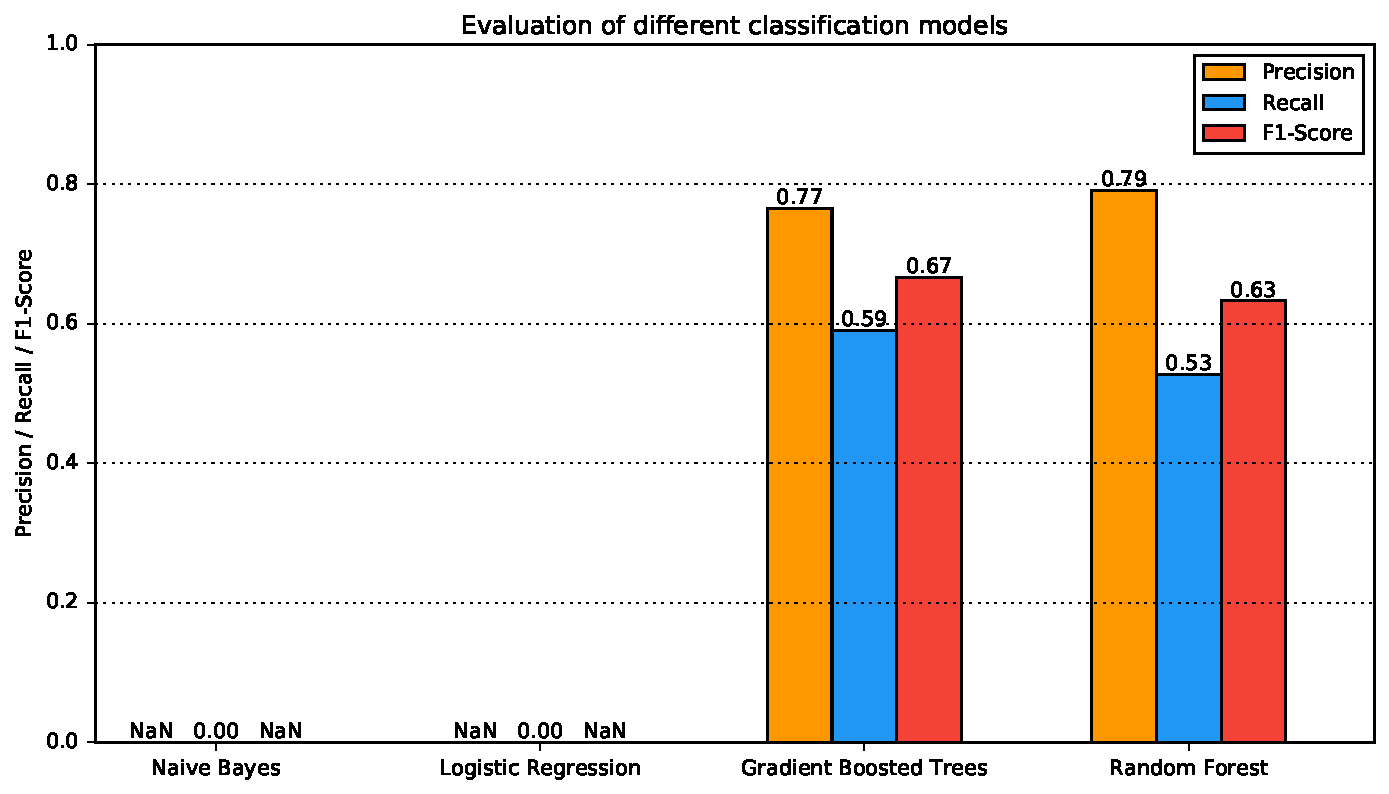
\includegraphics[width=\textwidth]{img/classifier_eval}
	\caption{Evaluation of different classification models.}
	\label{classifier_eval}
\end{figure}
Kurz erklären was man im Bild sieht\par
Naive Bayes
\begin{itemize}
	\item sagt immer nein
	\item nimmt an die features seien unabhängig, was sie nicht sind
	\item verschiedene Kostenmodelle getestet
\end{itemize}
Logistic Regression
\begin{itemize}
	\item sagt immmer nein
	\item verschiedene Kostenmodelle getestet
	\item Standard Paramter der Spark ML lib (und des Beispiels) benutzt
\end{itemize}
Gradient Boosted Trees
\begin{itemize}
	\item Standard Paramter der Spark ML lib (und des Beispiels) benutzt
\end{itemize}
Random Forest
\begin{itemize}
	\item vergleich DF und RDD API
	\item parameter getuned, haben aber nicht wirklich was geändert
	\item Kostenmodell kurve zeigen (für Seed und Candidate Alignments)
\end{itemize}
\begin{figure}[H]
	\centering
	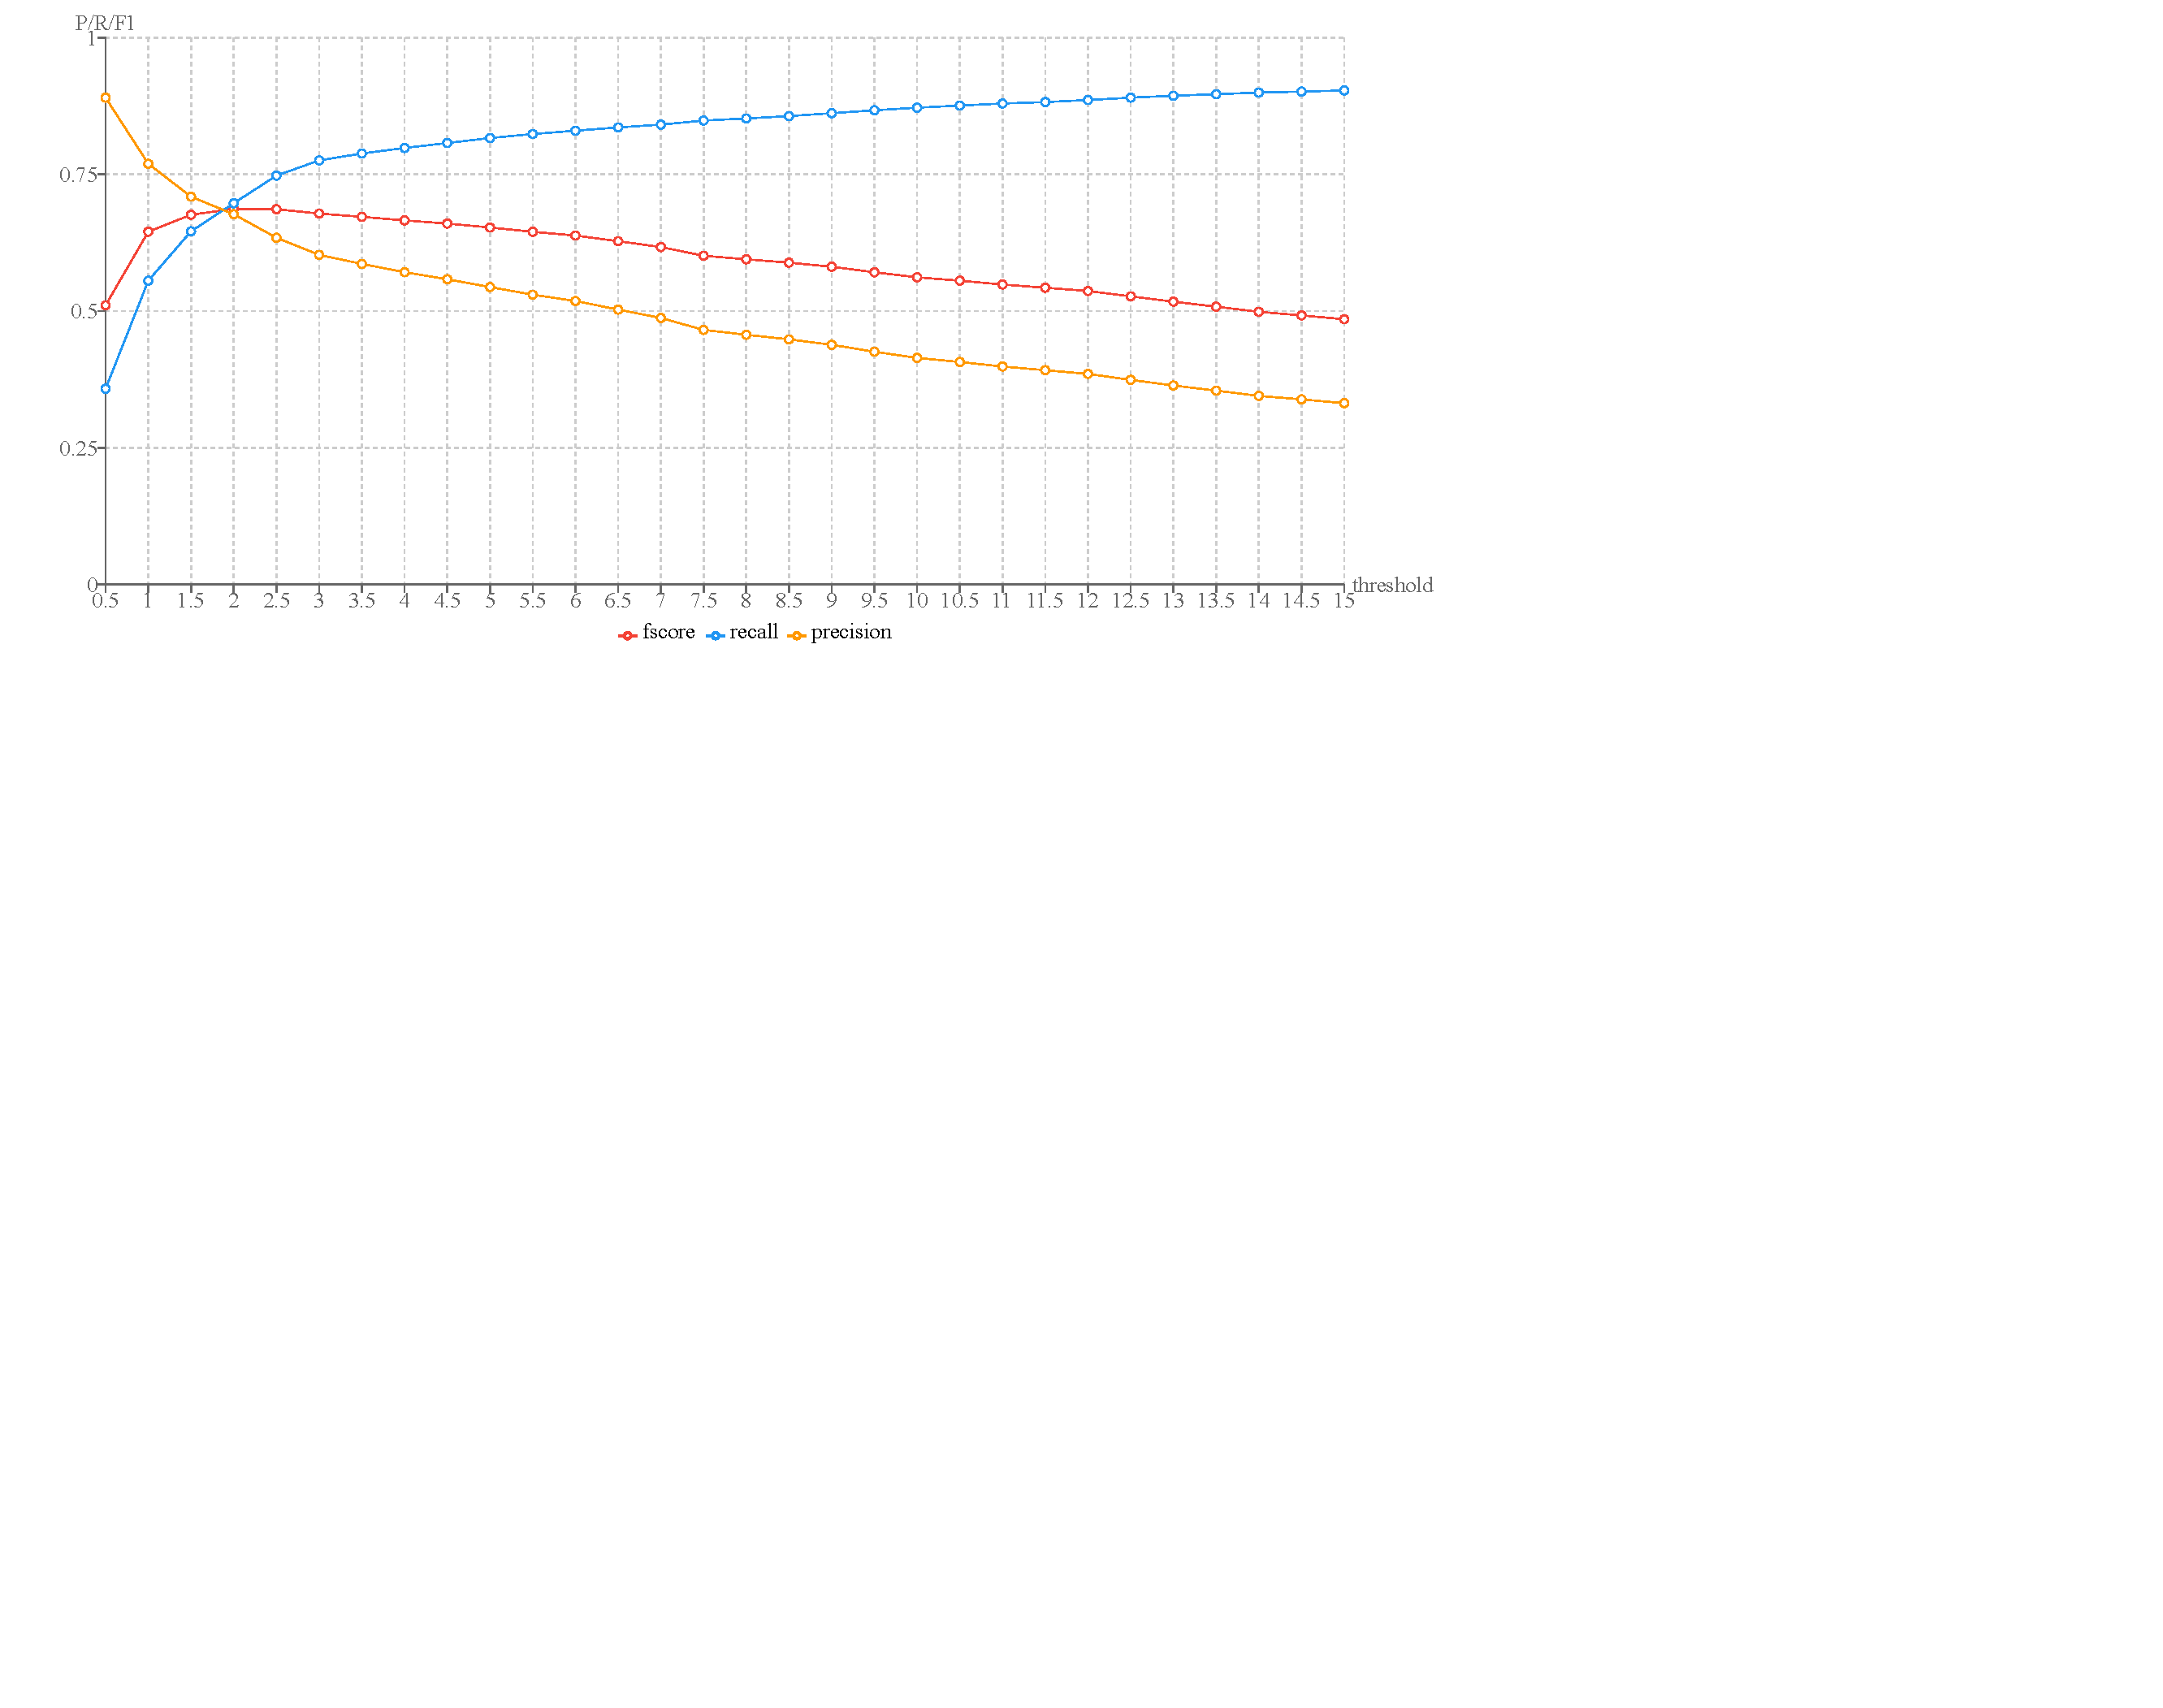
\includegraphics[width=\textwidth]{img/rf_thresh_large}
	\caption{Evaluation of different class weights of a random forest model.}
	\label{rf_thresh_large}
\end{figure}
\begin{figure}[H]
	\centering
	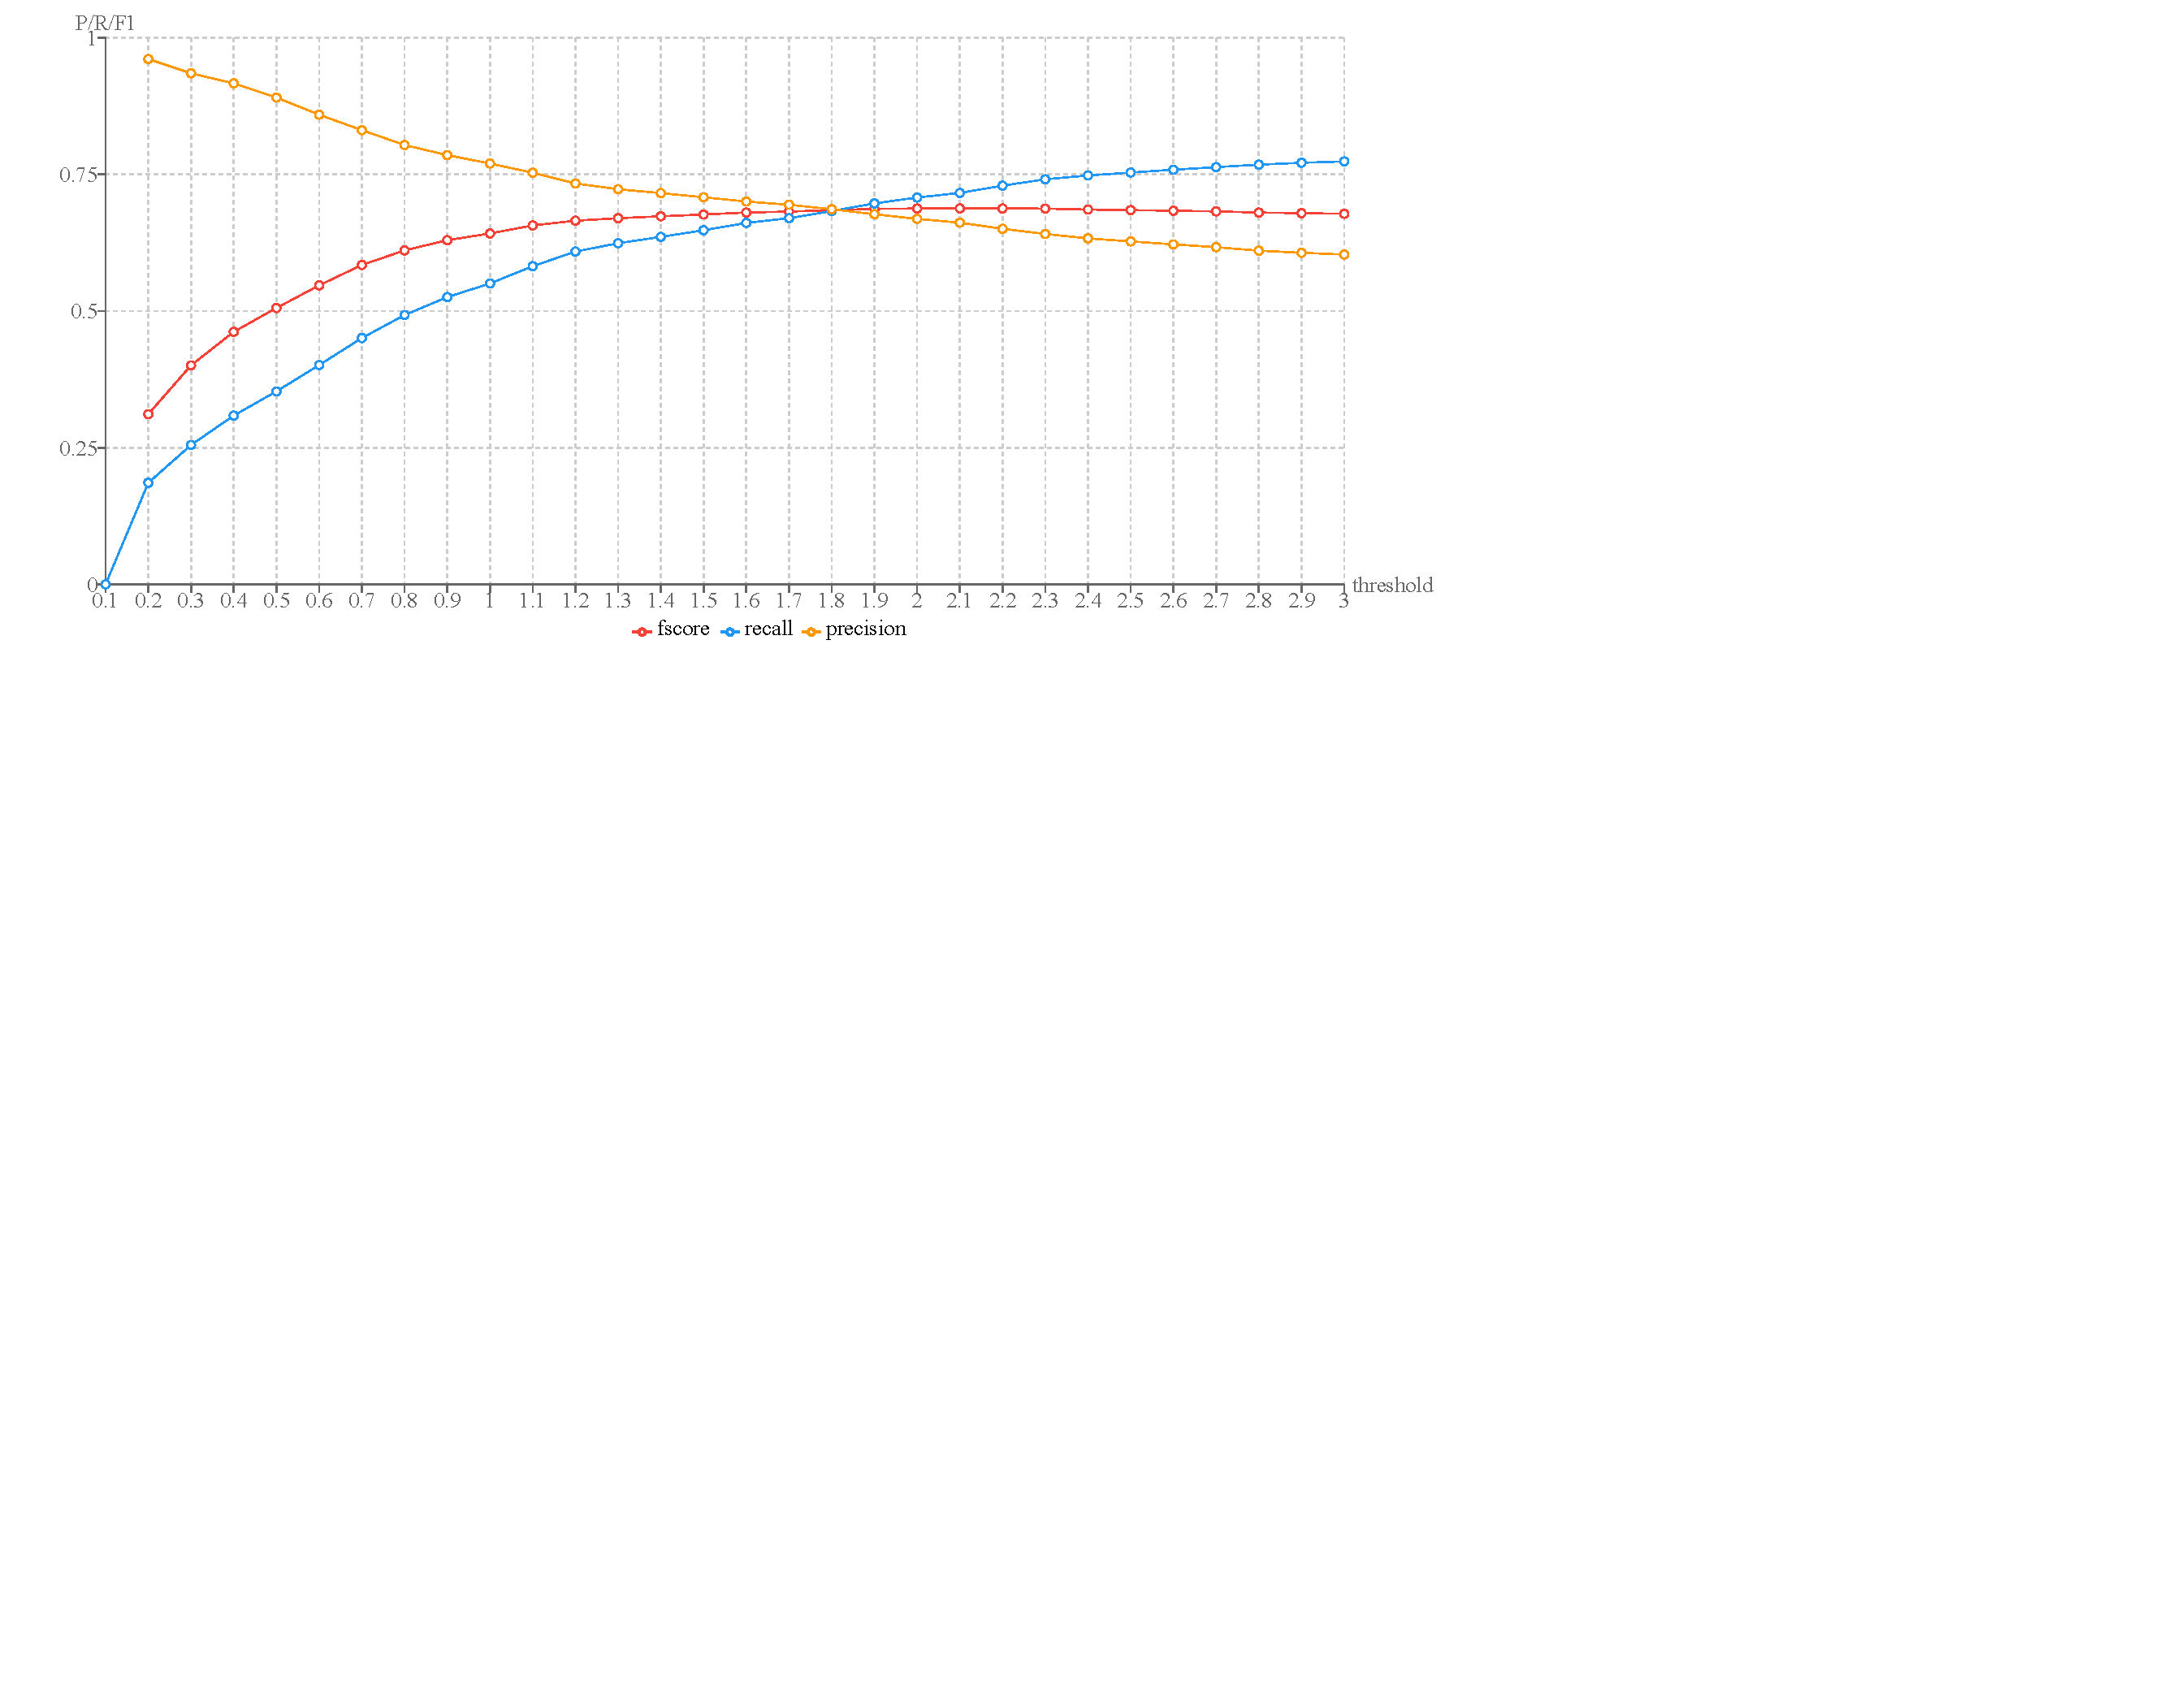
\includegraphics[width=\textwidth]{img/rf_thresh_small}
	\caption{Evaluation of different class weights of a random forest model.}
	\label{rf_thresh_small}
\end{figure}

% \begin{itemize}
% 	\item Evaluierungsmaß erklären\\
% 	Precision, Recall, F1-Score\\
% 	Precision mit bezug auf Mentions mit mehreren Alignments: $\frac{\text{Mentions mit mehreren Alignments}}{TP + FP}$
% 	\item aufzählen welche Classifier getesten werden:\\
% 	Naive Bayes, Random Forest, Logistic Regression, Gradient Boosted Trees, Support Vector Machines
% \end{itemize}
% 	\subsection{Classifier training and testing}
% 	\begin{itemize}
% 		\item Artikel von Unternehmen als Basis
% 		\item generieren Dateneinträge aus Wikipedia Links im Text, Extended Links und Trie Hits
% 		\item Simple Split (70/30) (bzw. noch mit Cross Validation machen)
% 		\item erwähnen dass RDD-API und DF-API der Spark ML andere Ergebnisse liefern
% 		\item (Standard Parameter der Spark ML erwähnen?)
% 	\end{itemize}

	% \subsection{Model Evaluation}
	% 	\subsubsection*{Naive Bayes}
	% 	\begin{itemize}
	% 		\item nicht gut, da die Features nicht unabhängig voneinander sind
	% 	\end{itemize}
	% 	\subsubsection*{Random Forest}
	% 	\begin{itemize}
	% 		\item erklären was man bei den Parametern (max Bins, max Depth, num Trees) erwarten
	% 		\item hat sich nicht viel geändert
	% 		\item Threshold Statistik zeigen für Seed und Candidate Alignments
	% 	\end{itemize}
	% 	\subsubsection*{Logistic Regression}
	% 	\subsubsection*{Gradient Boosted Trees}